% CS670 - Reinforcement Learning
% Dynamic Programming Assignment
% Gabriel Dulac-Arnold <gabe@squirrelsoup.net>
% Johannes H. Jensen <johannj@stud.ntnu.no>
\documentclass[a4paper]{article}
%\usepackage{multicol}
\usepackage{graphicx}
\usepackage[top=2cm,nohead,nofoot]{geometry}
\usepackage{subfig}



\graphicspath{{../graphs/}}

\author{Gabriel Dulac-Arnold $<$gabe@squirrelsoup.net$>$ (CS09F004) \\
Johannes H. Jensen $<$johannj@stud.ntnu.no$>$ (CS09F005)}
\title{CS670 - Reinforcement Learning \\
\emph{Dynamic Programming Assignment}}

\begin{document}
\setlength{\parskip}{2ex}
\maketitle

\section{Value Iteration}

Value iteration with $\theta=0.01$ produced the value functions plotted below. From the graph of the optimal $V^*$ we see that the best possible state is (0, 12, 0), that is 12 breedable cows.

\begin{figure}[ht]
\center
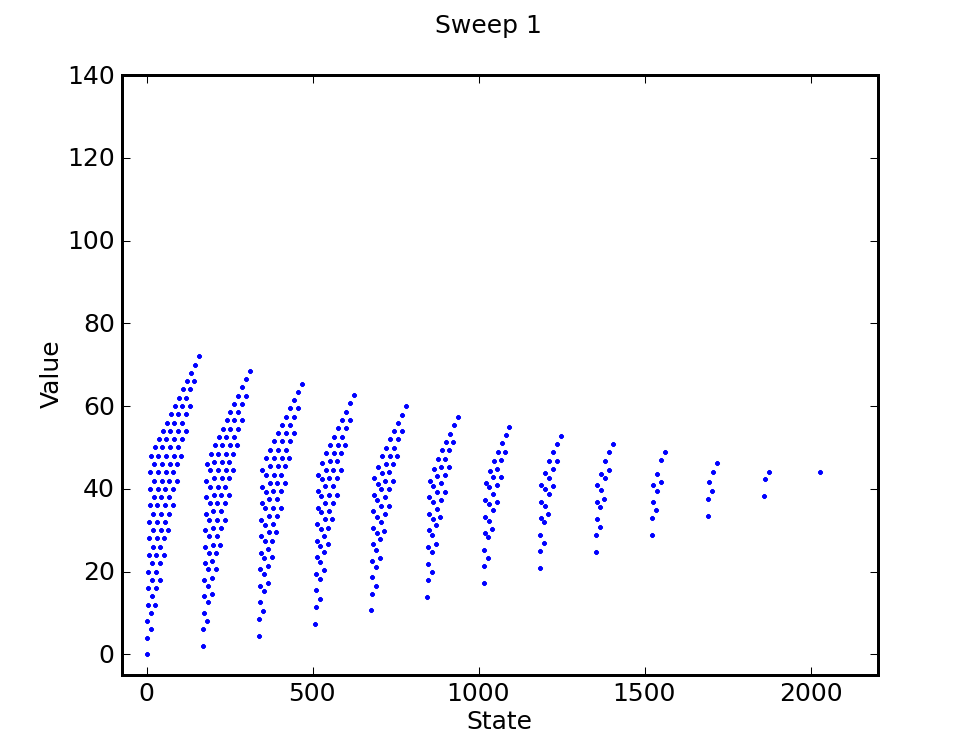
\includegraphics[scale=0.8]{value_iteration/sweep_1.png}
\caption{$V(s)$ after sweep 1}
\end{figure}

\begin{figure}[ht]
\center
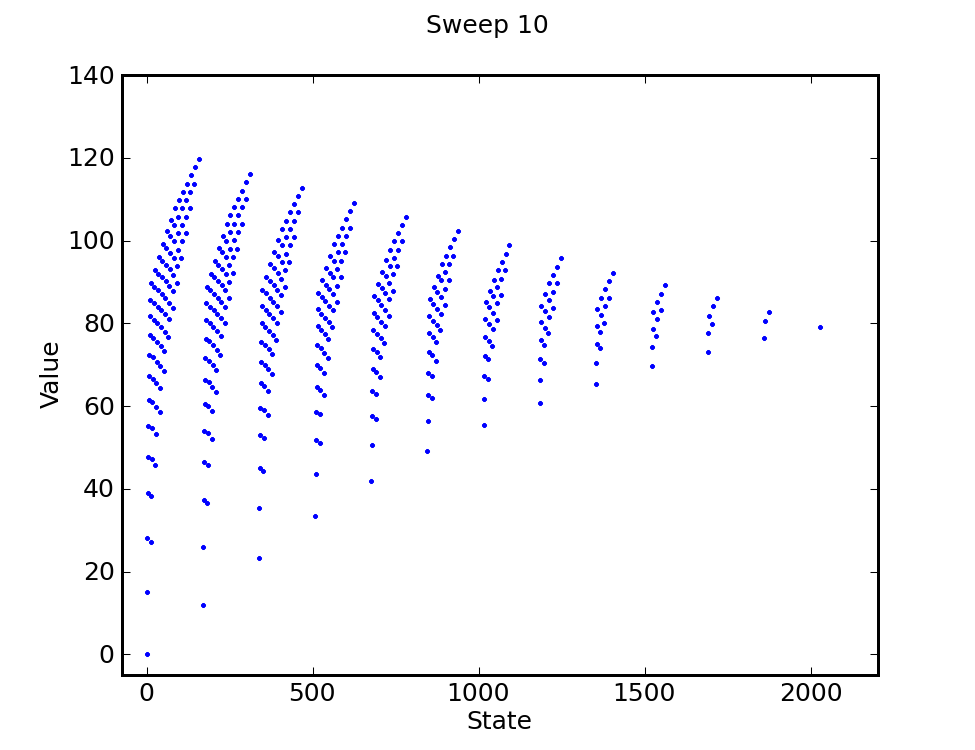
\includegraphics[scale=0.8]{value_iteration/sweep_10.png}
\caption{$V(s)$ after sweep 10}
\end{figure}

\begin{figure}[ht]
\center
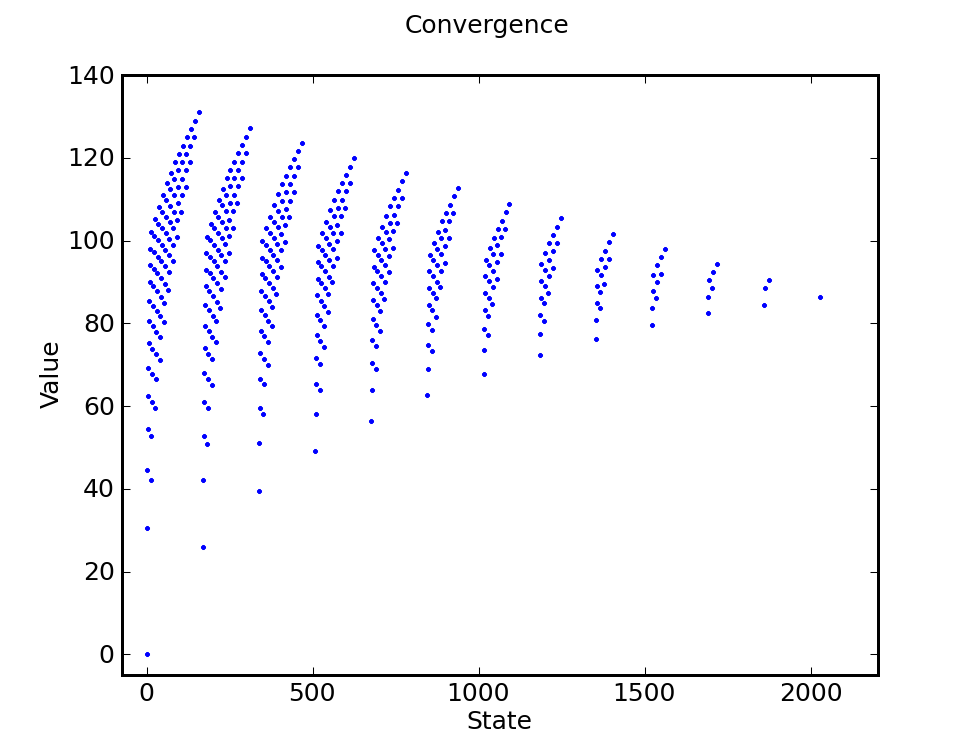
\includegraphics[scale=0.8]{value_iteration/convergence.png}
\caption{$V^*(s)$ at convergence}
\end{figure}


\clearpage

\section{Policy Iteration}

Policy Iteration with $\theta=0.01$ gave an optimal policy and value function
after 4 policy evaluations:

\begin{figure}[h]
\center
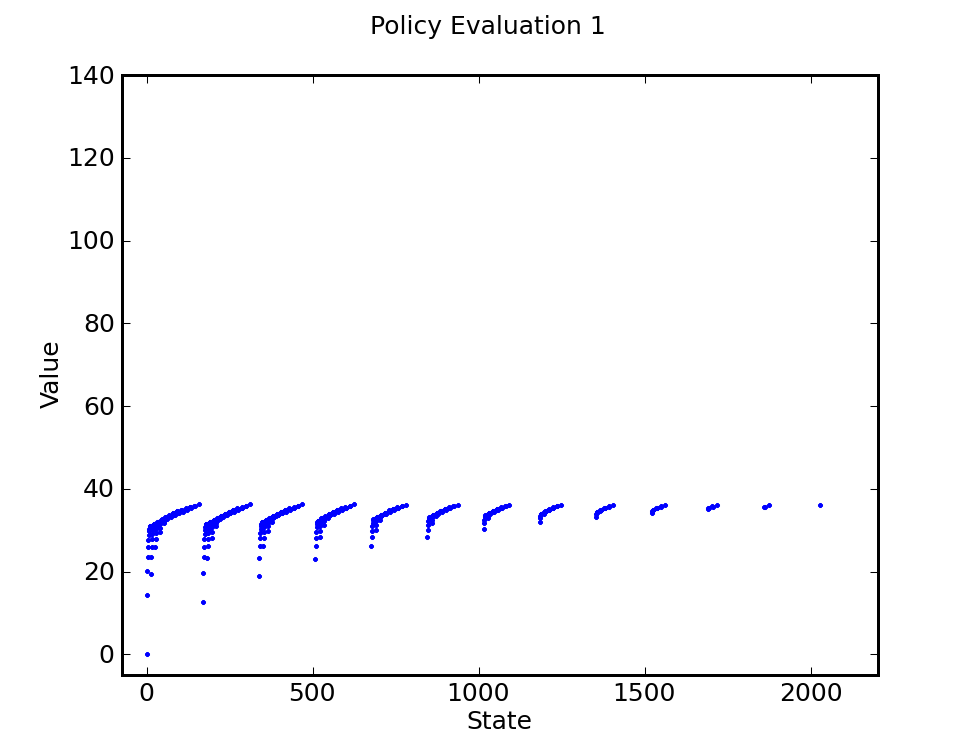
\includegraphics[scale=0.8]{policy_iteration/evaluation_1.png}
\caption{$V(s)$ after policy evaluation 1}
\end{figure}

\begin{figure}[h]
\center
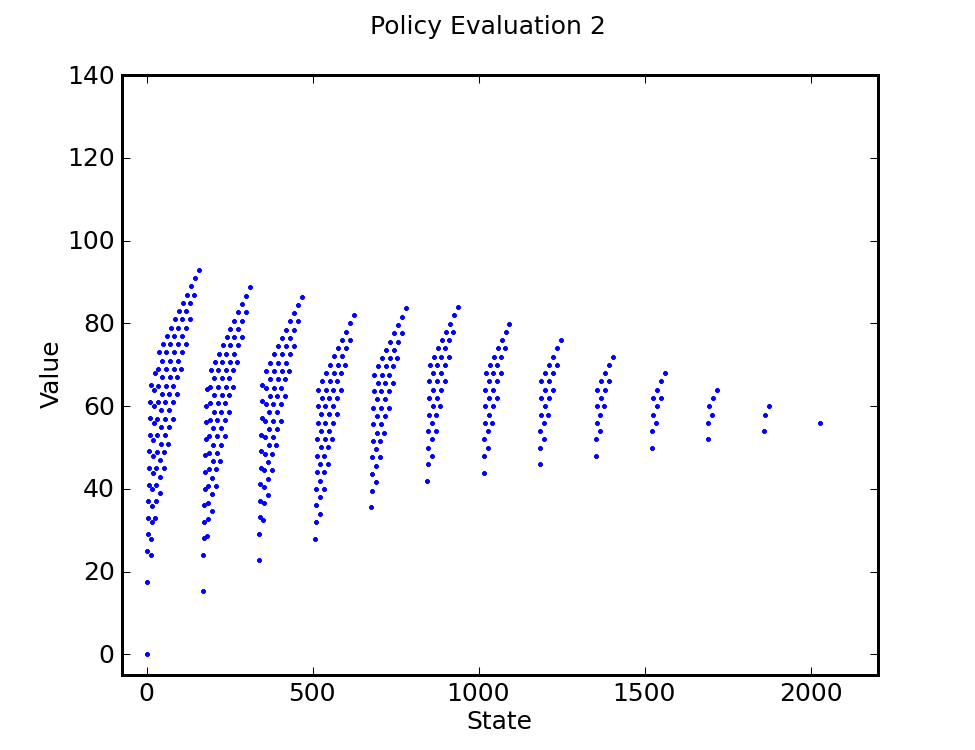
\includegraphics[scale=0.8]{policy_iteration/evaluation_2.png}
\caption{$V(s)$ after policy evaluation 2}
\end{figure}

\begin{figure}[h]
\center
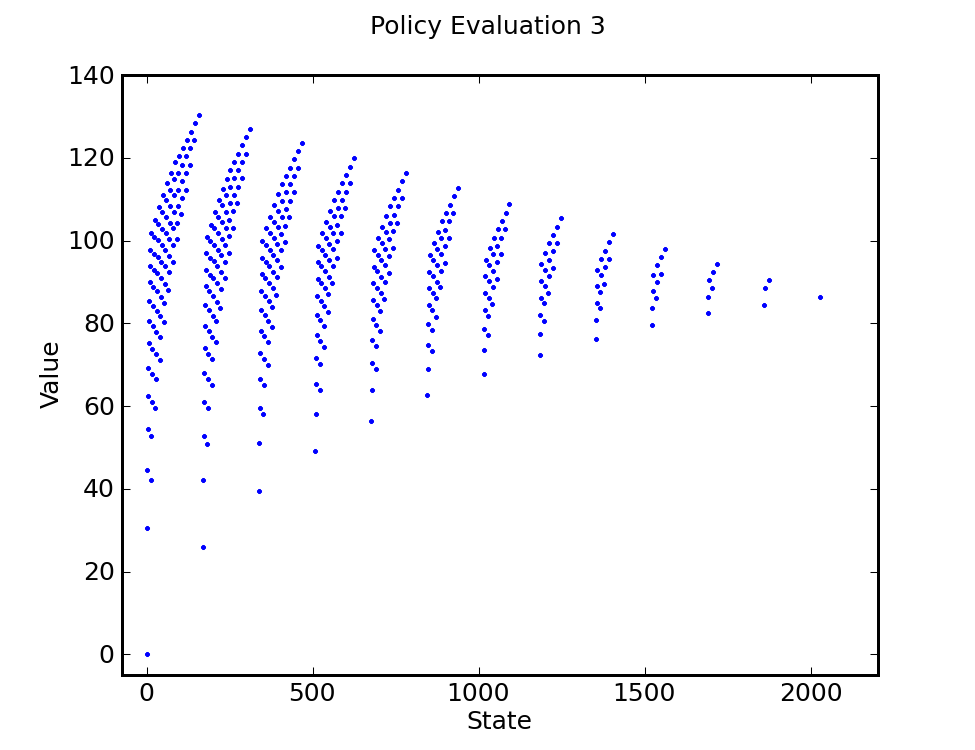
\includegraphics[scale=0.8]{policy_iteration/evaluation_3.png}
\caption{$V(s)$ after policy evaluation 3}
\end{figure}

\begin{figure}[h]
\center
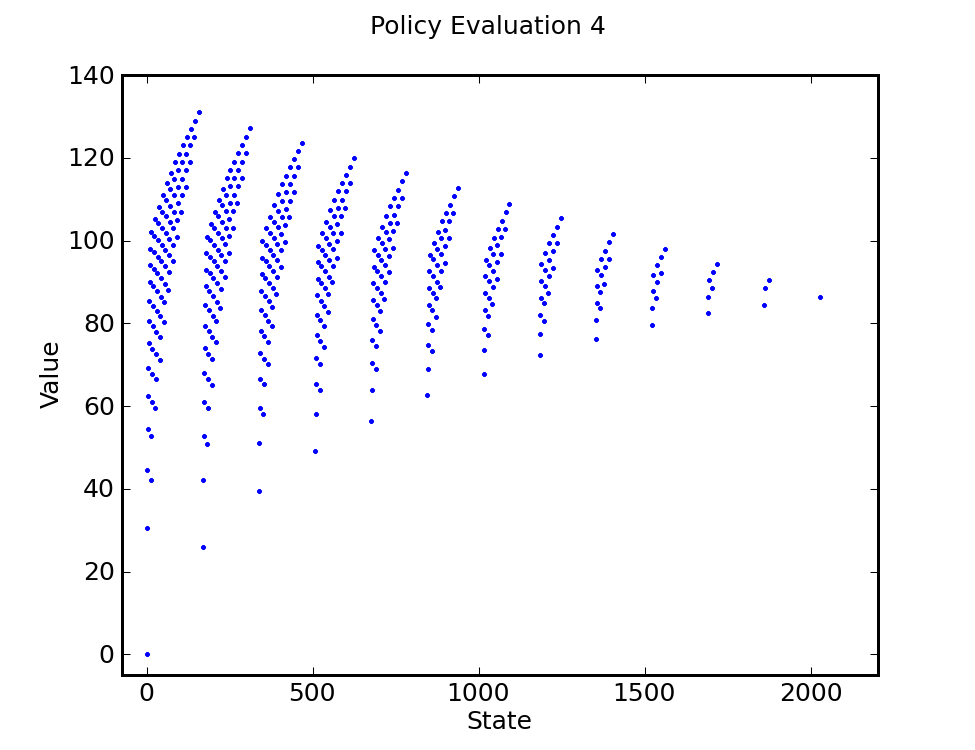
\includegraphics[scale=0.8]{policy_iteration/evaluation_4.png}
\caption{$V^*(s)$ after policy evaluation 4}
\end{figure}


\clearpage

\section{Varying the Discount Rate}

Policy Iteration with $\gamma = 0.5$ and $\gamma = 0.3$ converged after only 2 iterations of evaluation and improvement, whereas $\gamma = 0.9$ required 4 iterations to converge.
The smaller discount rates converge faster, but give much smaller values to the states.  This will have an important effect on the final policies (as we see later on).

\subsection{$V^*$ Plots}

%\begin{figure}
%  \centering
%  \subfloat[A gull]{\label{fig:gull}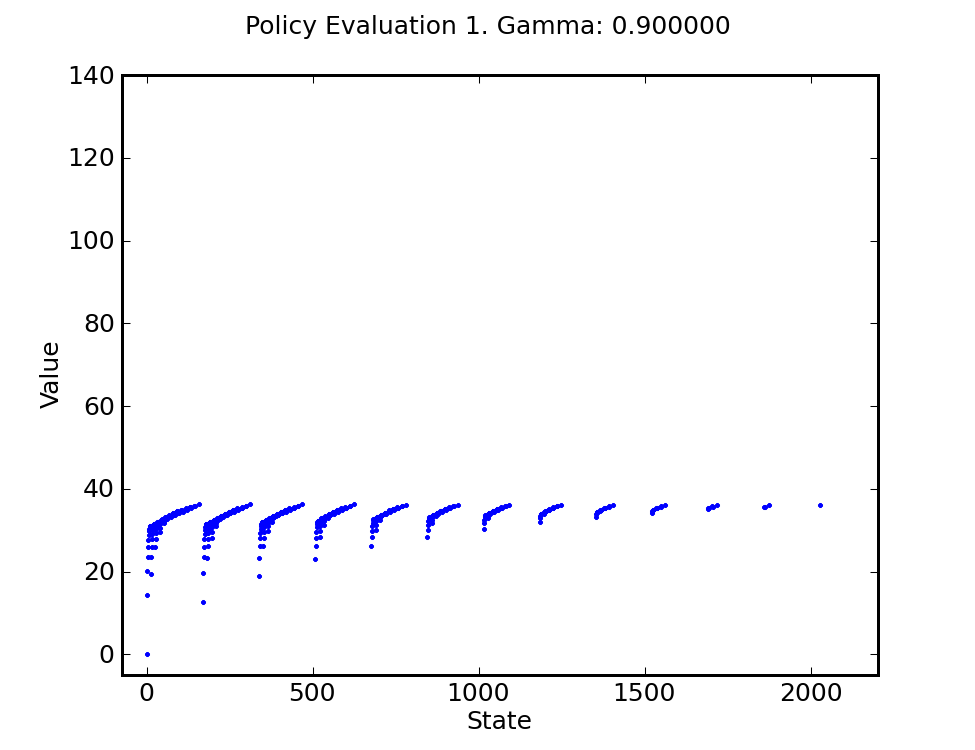
\includegraphics[width=0.3\textwidth]{gamma_iteration/gamma_9_1.png}}                
%  \subfloat[A tiger]{\label{fig:tiger}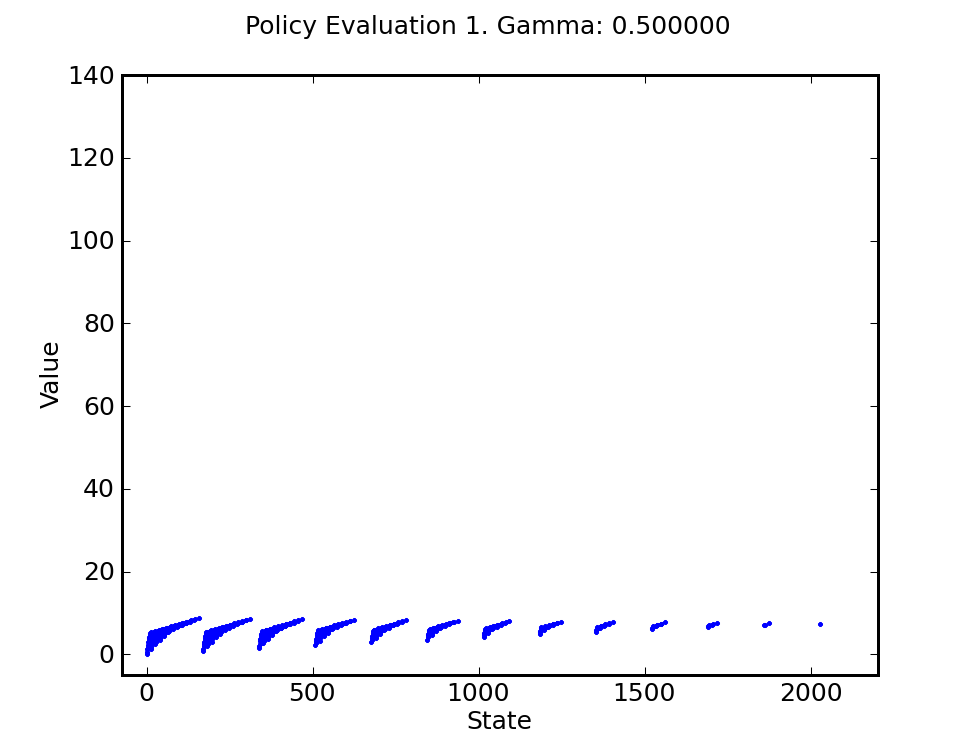
\includegraphics[width=0.3\textwidth]{gamma_iteration/gamma_5_1.png}}
%  \subfloat[A mouse]{\label{fig:mouse}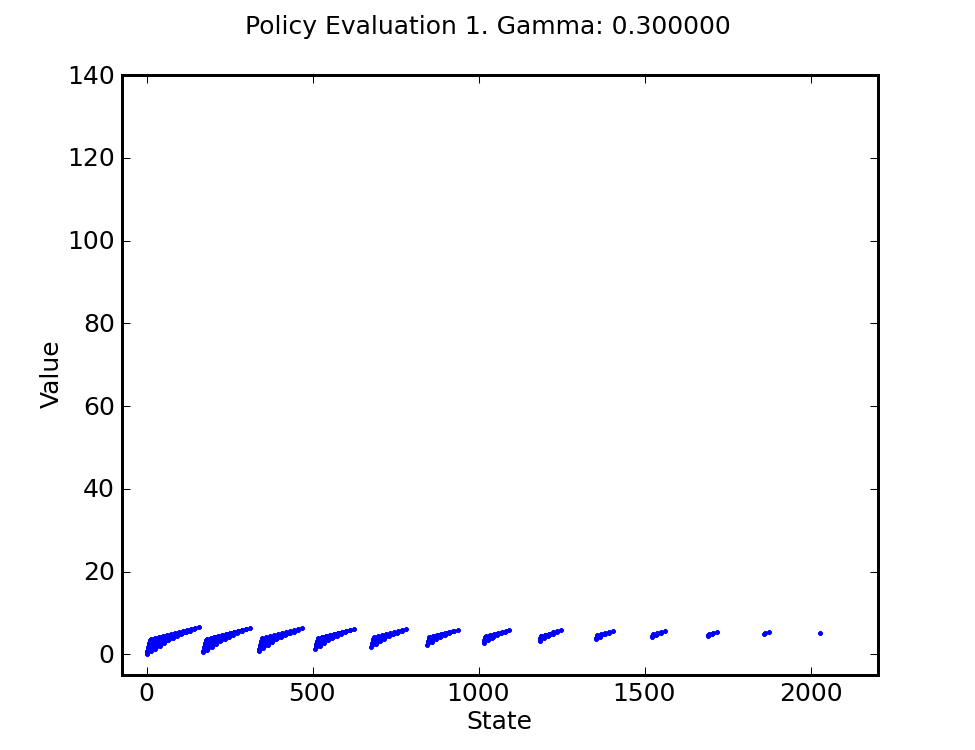
\includegraphics[width=0.3\textwidth]{gamma_iteration/gamma_3_1.png}}
%  \caption{Pictures of animals}
%  \label{fig:animals}
%\end{figure}

\begin{figure}[h]
\center
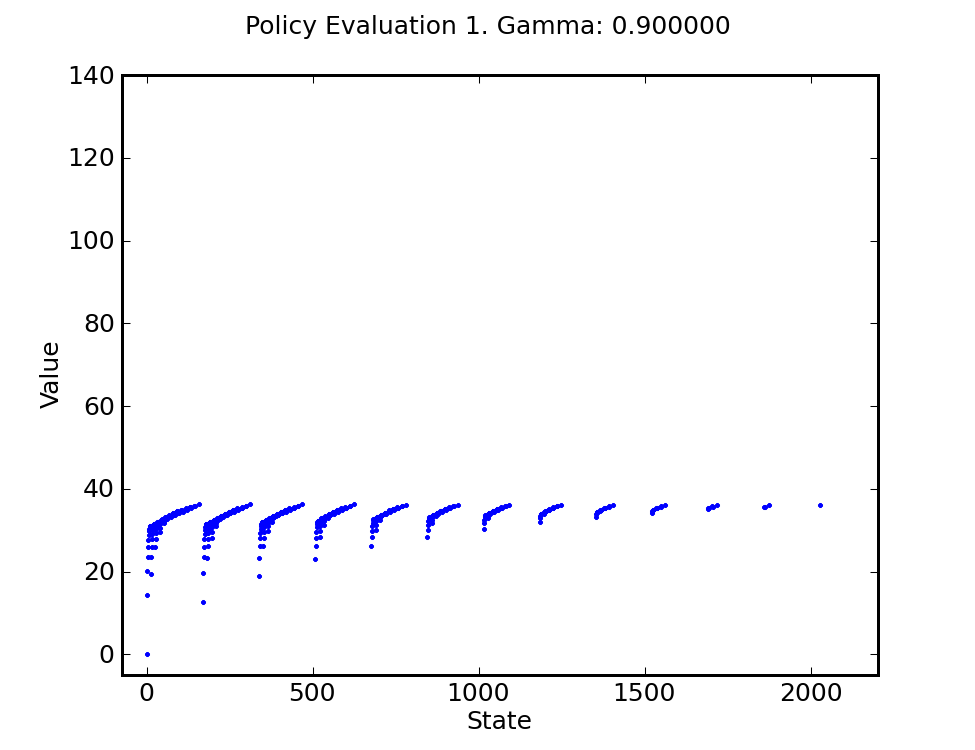
\includegraphics[scale=0.8]{gamma_iteration/gamma_9_1.png}
\end{figure}

\begin{figure}[h]
\center
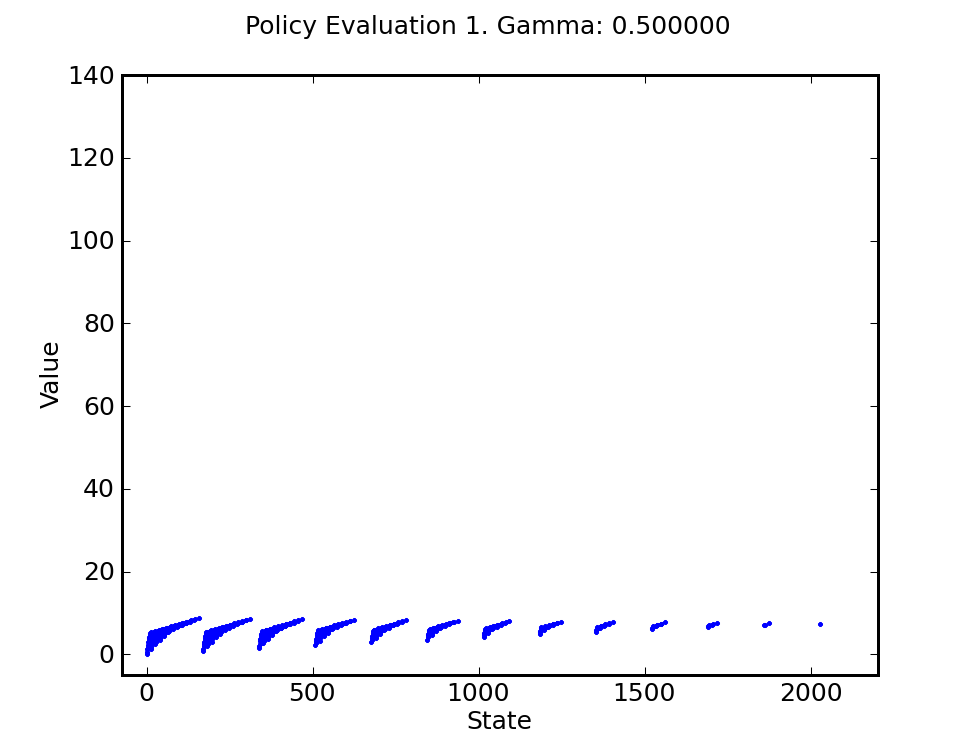
\includegraphics[scale=0.8]{gamma_iteration/gamma_5_1.png}
\end{figure}

\begin{figure}[h]
\center
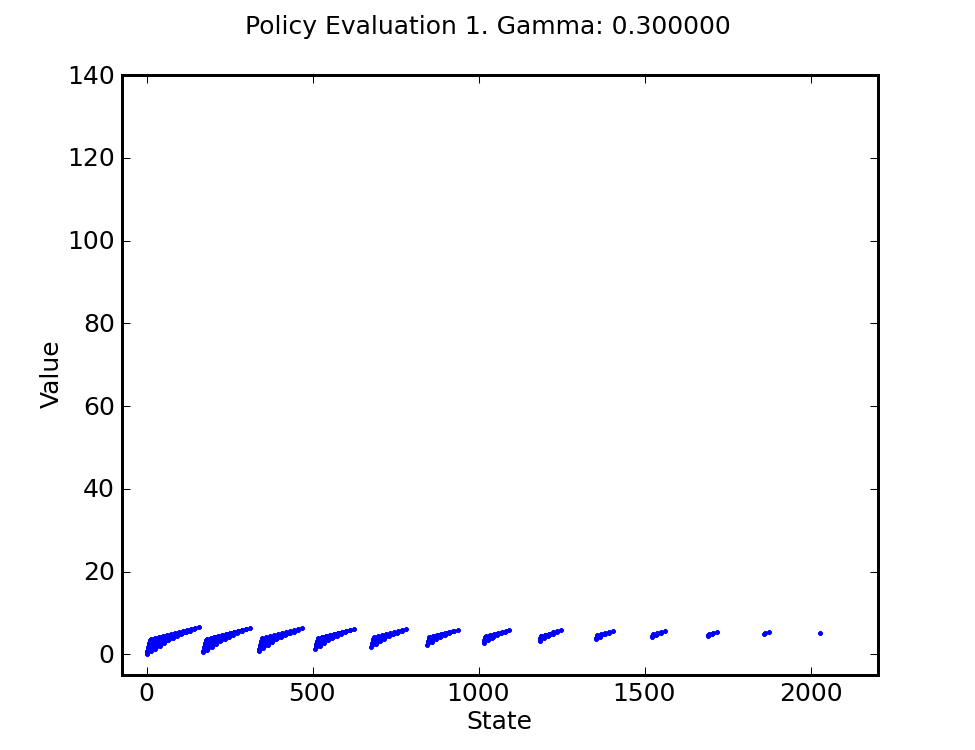
\includegraphics[scale=0.8]{gamma_iteration/gamma_3_1.png}
\end{figure}

\begin{figure}[h]
\center
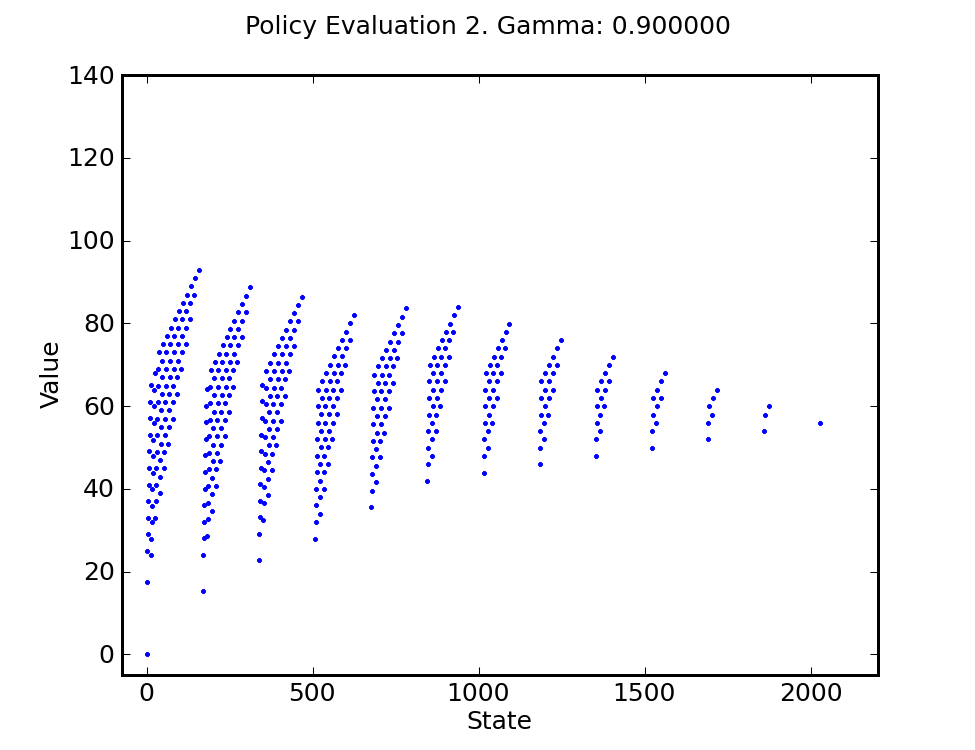
\includegraphics[scale=0.8]{gamma_iteration/gamma_9_2.png}
\end{figure}

\begin{figure}[h]
\center
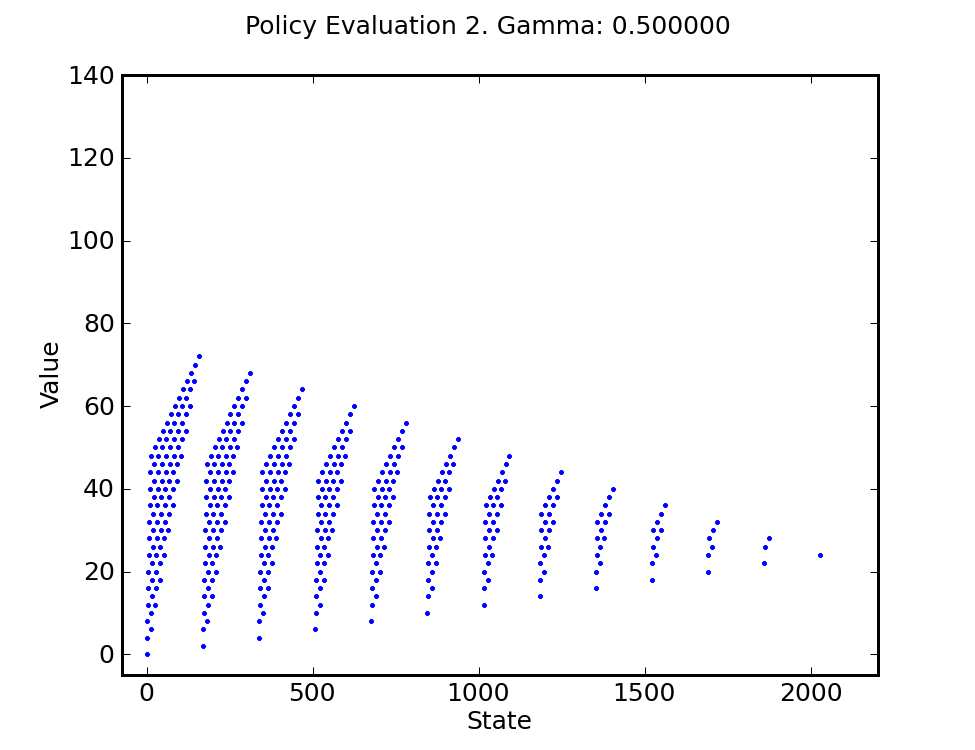
\includegraphics[scale=0.8]{gamma_iteration/gamma_5_2.png}
\end{figure}

\begin{figure}[h]
\center
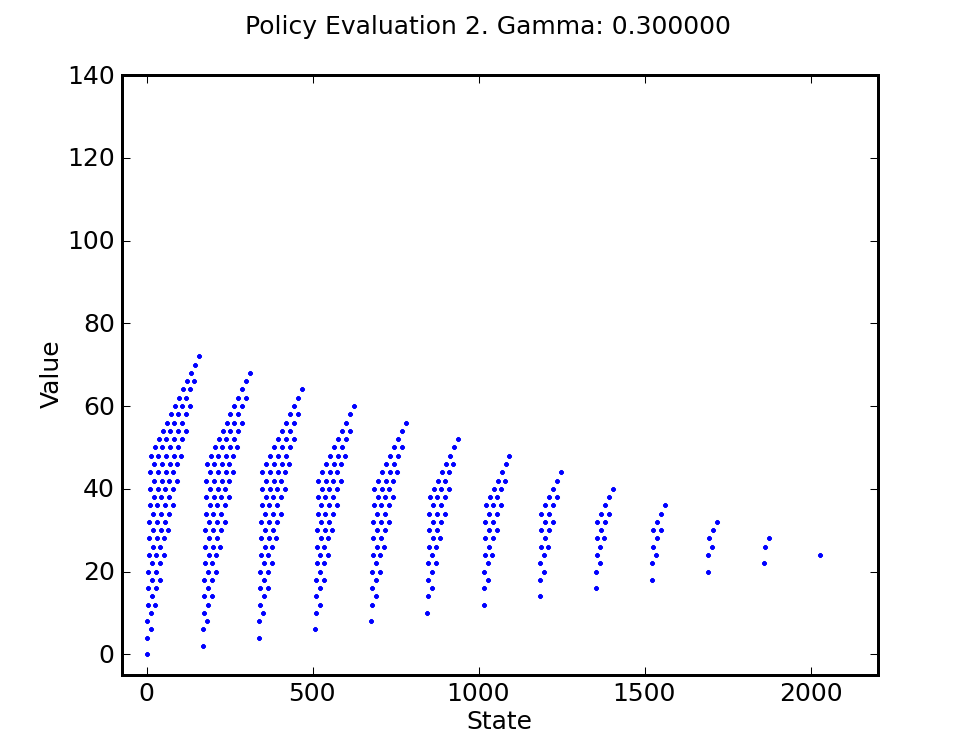
\includegraphics[scale=0.8]{gamma_iteration/gamma_3_2.png}
\end{figure}

\begin{figure}[h]
\center
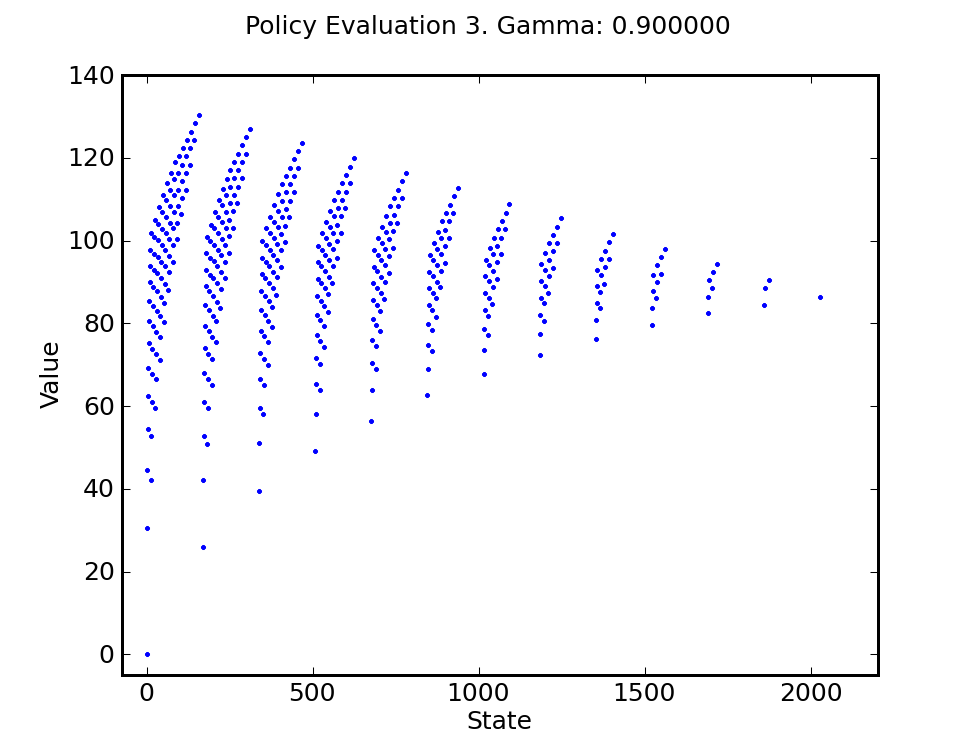
\includegraphics[scale=0.8]{gamma_iteration/gamma_9_3.png}
\end{figure}

\begin{figure}[h]
\center
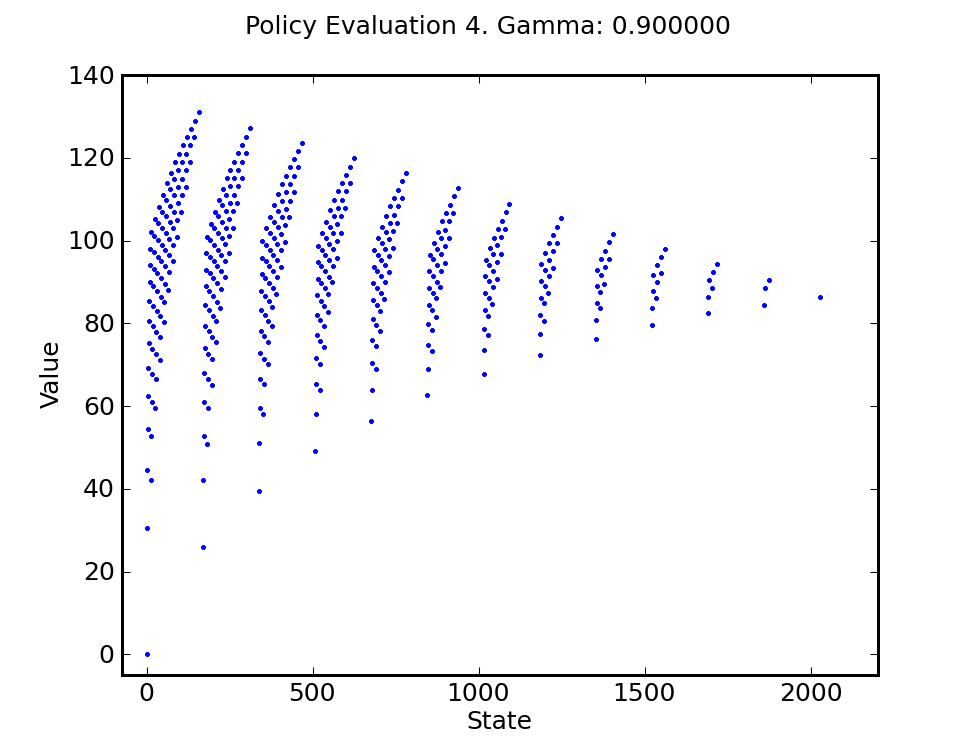
\includegraphics[scale=0.8]{gamma_iteration/gamma_9_4.png}
\end{figure}

\clearpage

\subsection{Policies}

The following table lists the optimal next action for the states (4, 7, 1), 
(1, 3, 6) and (9, 2, 1) with different values for $\gamma$:

\begin{tabular}{ l | c | c | c }
State $(y, b, o)$ & $\pi(s; \gamma = 0.9)$ & $\pi(s; \gamma = 0.5)$ & $\pi(s; \gamma = 0.3)$ \\
\hline
(4, 7, 1) & (0, 3, 1) & (4, 7, 1) & (4, 7, 1) \\ 
\hline
(1, 3, 6) & (0, 0, 2) & (1, 3, 6) & (1, 3, 6) \\
\hline
(9, 2, 1) & (0, 1, 1) & (9, 2, 1) & (9, 2, 1) \\
\end{tabular}

We can now see the problem with smaller values for $\gamma$. The immediate return for selling all the cows is not countered by big enough state values (
Because of this, policies for $\gamma = 0.5$ and $\gamma = 0.3$ are too greedy and result in the same bad action: sell all cows for immediate reward.
Policy iteration for $\gamma = 0.9$, however, produces a good policy for long-term cow farming.

\end{document}
